\documentclass[10pt]{article}
\usepackage{geometry}
\usepackage{multirow}
\usepackage{graphicx}
\usepackage{array}
\usepackage{amssymb}
\usepackage{amsmath}
\usepackage{enumitem}
\usepackage{listings}
\usepackage{float}
\usepackage[spanish]{babel}

\title{Tarea 5}
\author{Nicolas Aguilera García - 2127303}
\date{\today}
\geometry{letterpaper, top=2.5cm, bottom=2.5cm, left=3cm, right=3cm}    
\graphicspath{ {./images/} }
\setlength{\parindent}{0cm}
\setlength{\parskip}{0.2em}


\begin{document}
    \maketitle

    \section{Regla del trapecio}
    Para el desarrollo de este punto se definieron dos funciones principales, la primera es \texttt{trapezoidal\_rule} la cual toma como parámetro una función, el valor inicial y final desde donde evaluar y el número de iteraciones que se quiere realizar; la segunda función es \texttt{trapezoidal\_rule\_first\_5\_terms} la cual toma los mismos parámetros que la anterior función menos el número de iteraciones, ya que realiza la suma explicita de los primeros cinco términos.
    
    \begin{verbatim}
double trapezoidal_rule(function<double(double)> f, double a, double b, int N){
    double h, first_term, sum;
    
    h = (b - a) / N;
    first_term = (f(a) + f(b)) / 2;

    for (int i = 1; i < N; i++) {
        sum += f(a + i * h);
    }

    return h * (first_term + sum);
}

double trapezoidal_rule_first_5_terms(function<double(double)> f, double a, double b){
    double h, first_term, second_term, third_term, fourth_term, fifth_term;
    
    h = (b - a) / 5;
    first_term = (f(a) + f(b)) / 2;
    second_term = f(a + h);
    third_term = f(a + 2 * h);
    fourth_term = f(a + 3 * h);
    fifth_term = f(a + 4 * h);

    return h * (first_term + second_term + third_term + fourth_term + fifth_term);
}
    \end{verbatim}
    
    El valor de la integral se determinó para las siguientes funciones:
    
    \begin{table}[H]
        \centering
        \begin{tabular}{|c|c|c|}
        \hline
             & \textbf{Función} & \textbf{Rango} \\ 
        \hline
            a) & $3x$ & $[1, 2]$ \\
            b) & $x\cos^2 x + 1$ & $[0, \pi]$ \\
            c) & $3x + 4 e^x$ & $[0, 2]$ \\
        \hline
        \end{tabular}
        \caption{Funciones a las cuales se determinó el valor de la integral.}
        \label{tab:funciones}
    \end{table} 
    
    Los resultados del cálculo de la integral están dados por lo consignado en \ref{tab:valorintegral}.
    
    \begin{table}[H]
        \centering
        \begin{tabular}{|c|c|c|}
        \hline
            \textbf{Función} & \textbf{Forma del cálculo} & \textbf{Valor} \\ 
        \hline
            a)  & Analítico          & $4.5$ \\
            a)  & Numérico (n = 4)   & $4.5$ \\
            a)  & Numérico (n = 1)   & $4.5$ \\
            \hline
            b)  & Analítico          & $7.402203$ \\
            b)  & Numérico (n = 4)   & $7.4022$ \\
            b)  & Numérico (n = 2)  & $7.4022$ \\
            \hline
            c)  & Analítico          & $31.556224$ \\
            c)  & Numérico (n = 4)   & $31.8961$ \\
            c)  & Numérico (n = 140)  & $31.5567$ \\
        \hline
        \end{tabular}
        \caption{Valores de la integral evaluada mediante diferentes metodos.}
        \label{tab:valorintegral}
    \end{table}
    
    \section{Derivadas numéricas}
    Para el cálculo de las derivadas se definieron las siguientes funciones:
    
    \begin{verbatim}
double first_derivative(function<double(double)> f, double x, double h){
    return (f(x + h) - f(x)) / h;
}

double second_derivative(function<double(double)> f, double x, double h){
    return (f(x + h) - 2 * f(x) + f(x - h)) / pow(h, 2);
}
    \end{verbatim}
    
    Posteriormente, se ejecutaron las funciones anteriores para encontrar el valor de las derivadas numéricas con diferentes valores de $n$; se realizaron las gráficas utilizando el entorno \texttt{gnuplot} para leer/graficar los datos y generar las gráficas de las derivadas analíticas.
    
    \begin{figure}[H]
        \centering
        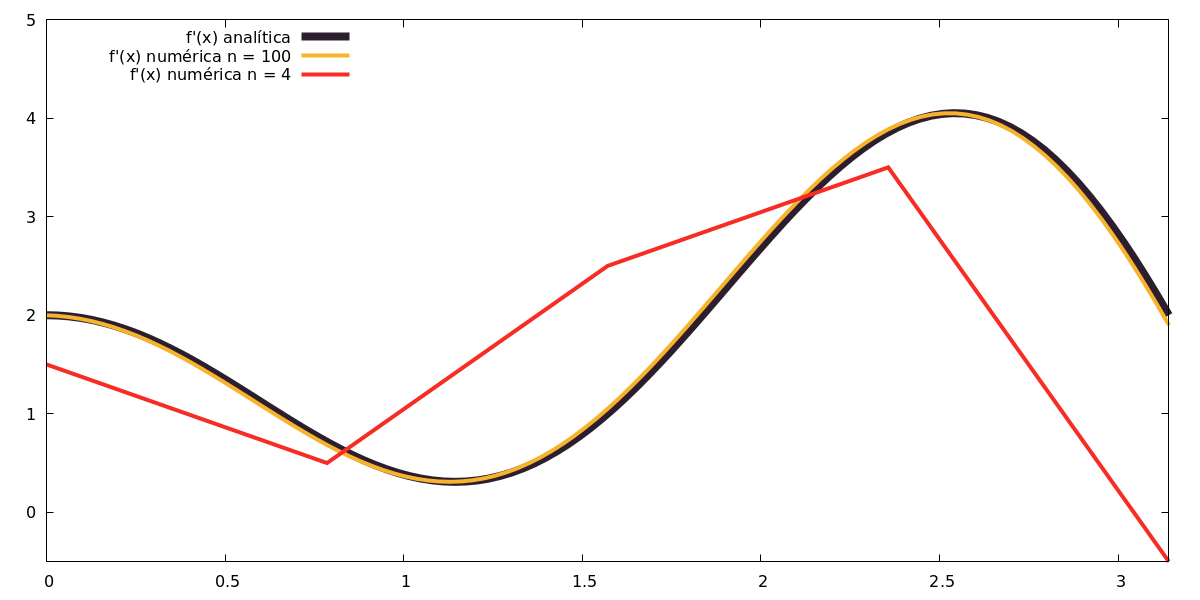
\includegraphics[scale=0.35]{images/derivadas-a.png}
        \caption{Gráfica primera derivada de $x\cos^2 x + 1$, expresión numérica cercana a analítica cuando $n=100$.}
        \label{img}
    \end{figure}
    
    \begin{figure}[H]
        \centering
        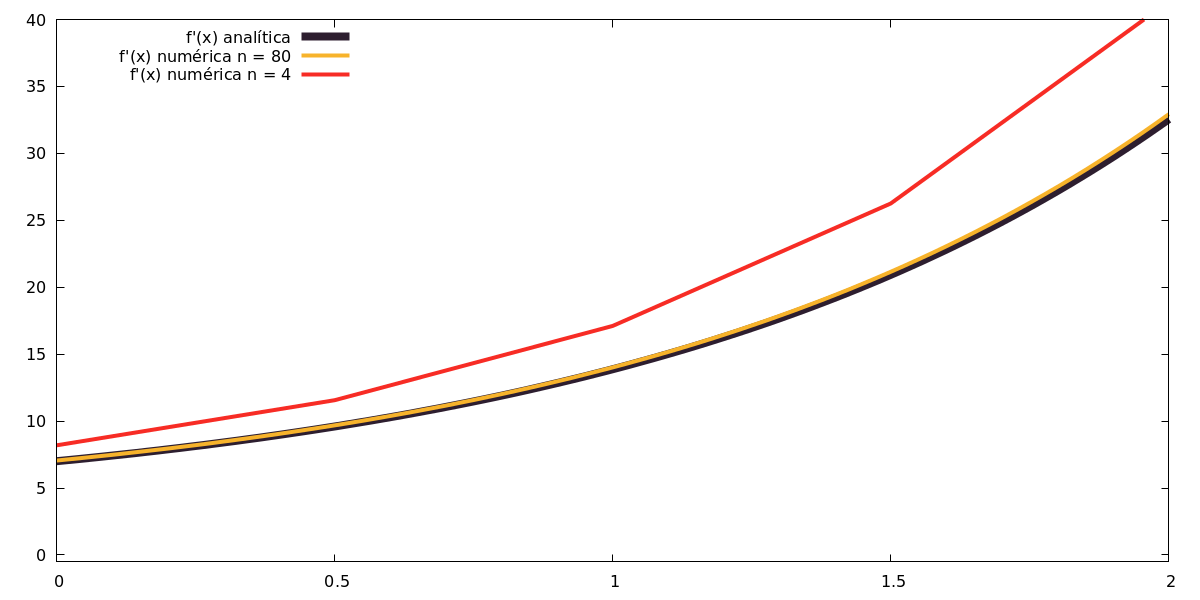
\includegraphics[scale=0.35]{images/derivadas-b.png}
        \caption{Gráfica primera derivada de $3x + 4 e^x$, expresión numérica cercana a analítica cuando $n=80$.}
        \label{img}
    \end{figure}
    
    \begin{figure}[H]
        \centering
        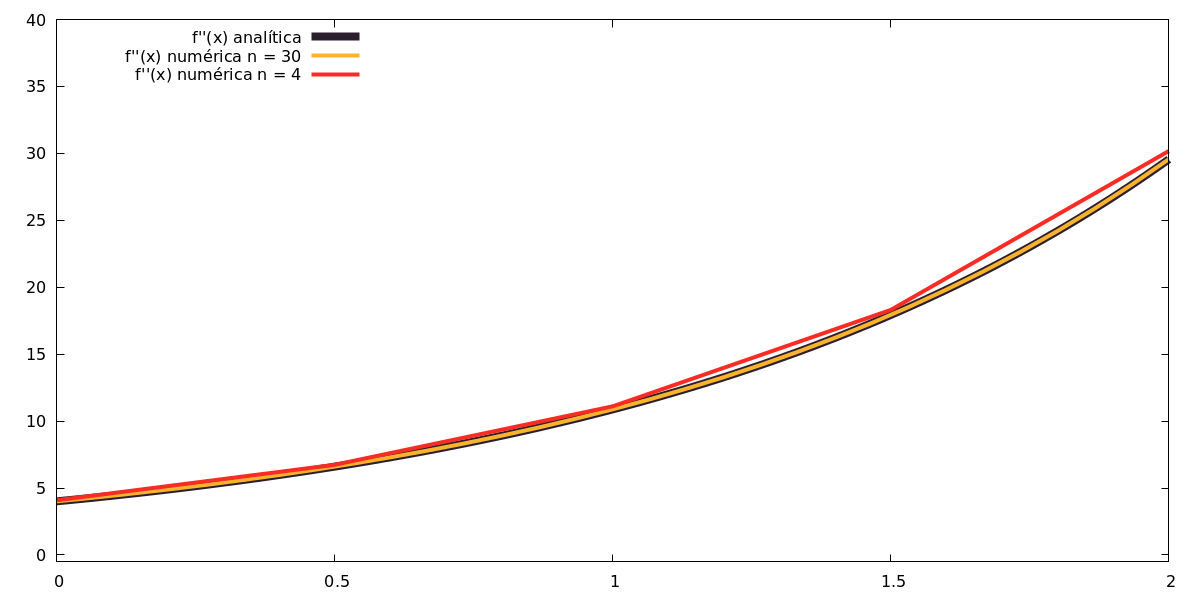
\includegraphics[scale=0.35]{images/derivadas-c.png}
        \caption{Gráfica segunda derivada de $3x + 4 e^x$, expresión numérica cercana a analítica cuando $n=30$.}
        \label{img}
    \end{figure}
    
    
    \section{Método Newton-Raphson}
    Se define la siguiente función polinómica junto con su derivada analítica:
    
    \begin{verbatim}
double f(double x){
    return 6 * pow(x, 3) - 3 * pow(x, 2) - 6 * x + 3;
}

double df(double x){
    return 18 * pow(x, 2) - 6 * x - 6;
}
    \end{verbatim}
    
    Tras esto se define una nueva función llamada \texttt{newton\_raphson} que se encargara de realizar el método acorde a los parámetros otorgados (valor inicial, tolerancia al error, función a evaluar y su derivada analítica).
    
    \begin{verbatim}
double newton_raphson(
    double x0,
    double tolerance,
    int N,
    function<double(double)> f,
    function<double(double)> df) 
{
    double x = x0;
    double fval = abs(f(x));
    int i = 0;

    while (fval > tolerance && i < N){
        x = x - f(x) / df(x);
        fval = abs(f(x));
        i++;
    }

    return x;
}
    \end{verbatim}
    
    Finalmente, se procede a ejecutar el código con los parámetros iniciales que se decidan, evidenciando que según el valor inicial elegido, el método encuentra uno u otro valor de $x$ que hace cero el polinomio.
    
    \begin{verbatim}
int main(){
    double x, x0, tolerance;
    int N;

    x0 = 0;
    N = 100;
    tolerance = 1e-6;

    x = newton_raphson(x0, tolerance, N, f, df);

    if (f(x) <= tolerance){
        cout << x << " --> " << f(x) << endl;
    }
    else{
        cout << "Solution does not converge." << endl;
    }


    return 0;
}
    \end{verbatim}
    
    
\end{document}